\section{Profiling the Method}
\label{sec:profiling}
The routine described for \ac{FID} estimation involves operations which can be
computationally demanding, with the burden on resources
increasing with the number of points in the \ac{FID}, as well as the number of
oscillators in the model. This is the case both in terms of the amount of work
done by the \ac{CPU}, and the amount of \ac{RAM} needed to store all the
required data as the routine runs. For the matrix pencil methods, the most
demanding aspect is performing \ac{SVD}, while for \ac{NLP}, it
is generation of the Hessian matrix for each iteration. Detailed accounts of the
computational complexity of the \ac{MPM} and \ac{MMEMPM} have been
presented~\cite{Hua1992,Chen2007}.  However, it is useful to consider what the
actual run times of these routines are on a modern computer; a lot of relevant
accounts are from decades before this work, and so the
run time will have decreased considerably thanks to
improvements in processing power. As an example, the account by Pines and
co-workers from 1997 outlining the \ac{ITMPM} states that a signal comprising
$1024$ points would take about
\qty{4.5}{\minute} to be processed by the \ac{MDL} and \ac{MPM}, using a
SGI Indigo workstation with \qty{100}{\mega\hertz} \ac{CPU}~\cite{Lin1997}. On
the system used for all results generated for this work (see
\cref{rem:workstation}) an equivalent computation takes about
\qty{100}{\milli\second}.
\correction{
    Furthermore, the consideration of larger datasets would have been
    impossible on the workstation used by Pines \emph{et~al}., which supported a
    maximal memory capacity of \qty{96}{\mebi\byte}; $N=1024$ is the largest
    power of 2 for which the required amount of storage for processing using
    the \ac{MPM} does not exceed \qty{96}{\mebi\byte}, as can be seen in
    \cref{fig:mpm-profiling}.a2.
}\label{corr:pines-ram}

To derive the results presented in this section, \Python\ implementations of
the aforementioned parts of the estimation routine were run, with software used
to assess both the line-by-line execution times~\cite{LineProf}, and the
time-dependent \ac{RAM} usage~\cite{MemProf}.
\begin{remark}
    \label{rem:workstation}
    All results presented in this work were acquired using a workstation
    featuring a Intel\textregistered\ Core\texttrademark\ i9-10900X \ac{CPU} @
    \qty{3.7}{\giga\hertz}, and \qty{32}{\gibi\byte} of \ac{RAM}.
\end{remark}

\subsection{The \acs{MPM} and \acs{MMEMPM}}
\label{subsec:mpm-profiling}
\begin{figure}
    \centering
    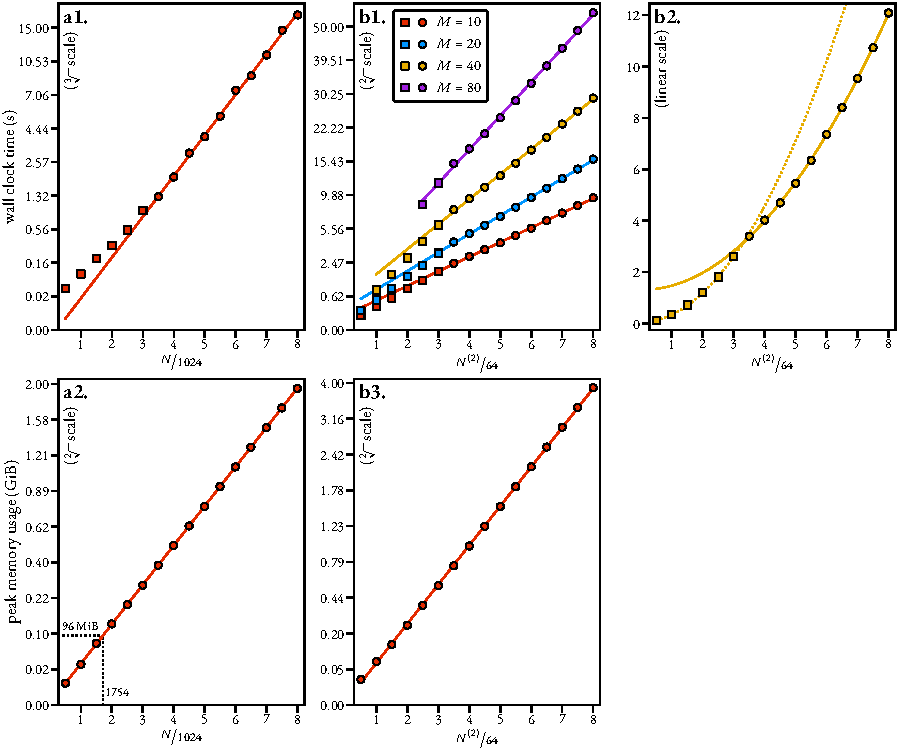
\includegraphics{mpm_profiling/mpm_profiling.pdf}
    \caption[
        The run time and peak memory consumption of
        the \acs{MPM} and \acs{MMEMPM}
        for \acsp{FID} with differing numbers of
        datapoints and constituent signals.
    ]
    {
        The \correction{wall clock time and peak memory usage} of
        the \acs{MPM} and \acs{MMEMPM}
        for \acsp{FID} with differing numbers of
        datapoints and constituent signals.
        The \acp{FID} that were used to acquire these results are described in
        the main text.
        \textbf{a1.} The amount of time required to compute the \ac{MPM}, as a
        function of number of points. Also plotted is a cubic fit of the
        circular points.
        \textbf{a2.} Peak memory consumption in performing the \ac{MPM} as a
        function of the number of points.
        \correction{
            The smallest number of datapoints
            that requires a least \qty{96}{\mebi\byte} of \ac{RAM} (1754) is
            indicated.
        }
        \textbf{b1.} The run time to compute the \ac{MMEMPM} of
        \acp{FID} with $\None = 64$, and variable $\Ntwo$ and $M$. Circular
        points have been fitted to quadratic functions.
        \textbf{b2.} The time required to compute the \ac{SVD} of $\EY$ for the
        $M=40$ \acp{FID}. The solid line is a quadratic fit of the circular
        points, while the dashed line is a quadratic fit of the square points.
        \textbf{b3.} Peak memory consumption in performing the \ac{MMEMPM} for
        the $M=40$ \acp{FID}.
    }
    \label{fig:mpm-profiling}
\end{figure}

A series of synthetic \ac{1D} \acp{FID} was constructed, comprising $10$ evenly-spaced
signals, with a
variable number of time-points $N \in \lbrace 512k : k \in \lbrace 1, 2, \cdots, 16 \rbrace \rbrace$.
For each \ac{FID}, the \ac{MPM} routine outlined in \cref{lst:mpm} was
performed 5 times.
The mean time to perform the \ac{MPM} across the 5 runs is plotted as a function
of $N$ in \cref{fig:mpm-profiling}.a1, where it can be seen that for
the larger values of $N$ considered, the \ac{MPM} is computed in approximately
$\mathcal{O}({N}^3)$ time;
a fit of a cubic function of the form $aN^3 + b$ to the data satisfying $7 \leq
k \leq 16$ is plotted to highlight this.
The cubic dependence is realised since the rate-limiting step of the
\ac{MPM} is \ac{SVD} of $\Hy$, whose size is to a very good approximation
$\tfrac{2N}{3} \times \tfrac{N}{3}$\footnote{
    \label{fn:svd-complexity}
    The time complexity for the \ac{SVD} of generic a $m \times n$ matrix is
    $\mathcal{O}(\operatorname{min}(m, n)^2 \cdot \operatorname{max}(m, n))$,
    while the space complexity is $\mathcal{O}(mn)$.
}. For smaller values of $N$, a deviation
away from a cubic relationship is observed.
This arises because the computation of the complex amplitudes using
\cref{eq:complex-amplitudes} has a comparatively significant run time
relative to \ac{SVD} in the low-$N$ regime;
for a $512$ point signal, \ac{SVD} of $\Hy$ took up roughly 80\% of the
complete run time, while the computation of the complex amplitudes took up
roughly 20\%. For a 8192 point signal, these percentages had changed to
$>\!\!99\%$ and $<\!\!1\%$, respectively.

The \ac{MPM} was run once more on each generated \ac{FID} in order to assess
the effect of $N$ on the space complexity.
The peak \ac{RAM} consumption is plotted in \cref{fig:mpm-profiling}.a2.
A clear quadratic dependence on consumption is realised as function of $N$,
again in agreement with the expected space complexity of the
\ac{SVD}\footnoteref{fn:svd-complexity}.

A similar study was conducted for the consideration of the \ac{MMEMPM}. A
series of hypercomplex \ac{2D} \acp{FID} were simulated, all of which all
comprised $\None = 64$. The \acp{FID} possessed values of $\Ntwo \in \lbrace
32k : k \in \lbrace 1, \cdots, 16 \rbrace \rbrace$.
With the \ac{MPM}, since a complete \ac{SVD} of the matrix $\Hy$ is computed,
the model order is irrelevant in dictating the run time (at least when $M \ll
N$). This is not the case for the \ac{MMEMPM}; because the \Python
implementation used (\cref{lst:mmempm}) employs a truncated \ac{SVD} in order
to compute only the first $M$ components of $\EY$, the elected model order will
have an impact on run time.  Therefore, \acp{FID} with different model orders
were generated: $M \in \lbrace 10, 20, 40, 80 \rbrace$.

The \ac{MMEMPM} was repeated 5 times for each \ac{FID}, and the mean run
times for each $\Ntwo$ and $M$ considered is plotted in
\cref{fig:mpm-profiling}.b1.
Results are only presented in cases where the \ac{MMEMPM} was able to yield a
satisfactory estimation result in close agreement with the model used to
generate the \ac{FID}; for certain \acp{FID} with low
$\Ntwo$ and high $M$, appropriate estimation results could not be obtained as
the constituent signals were too poorly resolved.
While in the high-$N$ regime the \ac{MPM} has a cubic time dependence
on the number of points, the \ac{MMEMPM} can be seen to have an approximately
quadratic complexity regarding $\Ntwo$.
For all combinations of $\Ntwo$ and $M$,
the truncated \ac{SVD} was the most time consuming aspect of the routine,
however other steps have notable run times too. The \ac{MMEMPM} can be broken
down into the following 5 steps, with the relevant lines in \cref{lst:mmempm}
given:
\begin{enumerate}
    \item Construction of $\EY$. This involves building the Hankel matrices
        $\lbrace \symbf{H}_{\symbf{y},\none} : \none \in \lbrace 0, \cdots, 63
        \rbrace \rbrace$, assigning them to the
        correct locations in $\EY$, and finally converting  $\EY$ to a sparse
        matrix\footnote{
            Truncated \ac{SVD} is only available for sparse matrices in
            \textsc{NumPy}~\cite{svds}. Some experimenting was done to determine
            the most efficient means of generating $\EY$ in sparse form, and
            subsequently compute its \ac{SVD}.
            It was determined that constructing $\EY$ using a
            standard \textsc{NumPy} array before converting it to
            \ac{CSR} format~\cite{csr} was optimal.
            \label{fn:sparse-svd}
        } (Lines \ref{ln:EYstart} to \ref{ln:EYend}).
    \item Truncated \ac{SVD} of $\EY$ to generate $\symbf{U}_M$ (Line \ref{ln:sparse2}).
    \item Determining $\bdzone$ and  $\symbf{W}^{(1)}$ by computing the
        eigenvalue decomposition of $\symbf{U}_{M1}^+ \symbf{U}_{M2}^{\vphantom{+}}$ (Lines
        \ref{ln:poles1start} to \ref{ln:poles1end}).
    \item Generating the second set of signal poles $\bdztwo$, by
        multiplying $\symbf{U}_M$ with the permutation matrix, and extracting
        the diagonal from matrix $\symbf{G}$, computed using \cref{eq:G} (Lines
        \ref{ln:poles2start} to \ref{ln:poles2end}). N.B. The \acp{FID} were
        constructed such that the signal poles were unique on all occasions, so
        the additional treatment of repeated signal poles was not necessary.
    \item Computation of the complex amplitudes using
        \cref{eq:complex-amplitudes-2d} (Lines \ref{ln:compamps2dstart} to
        \ref{ln:compamps2dend}).
\end{enumerate}
A comparison of the relative times to perform these steps for some select
pairings of $M$ and $\Ntwo$ is provided by \cref{tab:mmempm-steps}. It can be
seen that as $M$ increases, the relative amount of time spent performing
\ac{SVD} increases, while that to generate $\EY$ decreases. This
reflects the greater number of iterations required by
the truncated \ac{SVD} routine~\cite{svds} to produce the desired number of
components, while the run time to generate $\EY$ remains fixed.

Interestingly, the plots for a given value of $M$ in
\cref{fig:mpm-profiling}.b1 do not exhibit
consistent quadratic behaviour throughout; after a certain value of $\Ntwo$, a
slight reduction in the gradient of the plots is observed (cf
the square and circular points). This was found to be caused by the \ac{SVD}
computation, whose run times for the $M=40$ \acp{FID} are plotted in
\cref{fig:mpm-profiling}.b2.
The square and circular points both display quadratic behaviour, though the
exact form of the function which
describes them are different; both sets of points have been fit to curves of
the form $a\Ntwo^2 + b$. After $\Ntwo$ becomes larger than
roughly $200$, the \ac{SVD} run time appears to enter a new regime in which
a slower rate of increase is observed. The exact reason for why this is
observed was not ascertained.

The peak \ac{RAM} usage for the $M=40$ \acp{FID} as a function of $\Ntwo$ is
plotted in \cref{fig:mpm-profiling}.b3, where a quadratic complexity is
observed. The variation in memory consumption barely changes as a function of
the model order, since the peak usage is largely dependent on the size of
$\EY$.

It should be noted that the run time and peak \ac{RAM} consumption will also be
(roughly) quadratically dependent on $\None$, just as with $\Ntwo$, e.g.
increasing  $\None$ from  $64$ to $128$ would cause all the run times and peak
memory usages in Figures \ref{fig:mpm-profiling}.b1 and
\ref{fig:mpm-profiling}.b3 to quadruple in value.

\begin{table}
    \begin{center}
        \begin{tabular}{ c c c c c c c }
            \toprule
            $\Ntwo$ &
            $M$ &
            Step 1 &
            Step 2 &
            Step 3 &
            Step 4 &
            Step 5 \\
            \midrule
            64 & 10 & 12.2\% & 60.6\% & 2.9\% & 9.7\% & 13.8\% \\
            64 & 40 & 4\% & 74.6\% & 1.9\% & 8.9\% & 9.6\% \\
            512 & 10 & 22.1\% & 67.2\% & 0.2\% & 3.1\% & 7.2\% \\
            512 & 40 & 7.4\% & 81.9\% & 0.1\% & 1.3\% & 9.4\% \\
            512 & 80 & 3.8\% & 85.8\% & 0.1\% & 0.8\% & 9.4\% \\
            \bottomrule
        \end{tabular}
    \end{center}
    \caption[
        A comparison of the relative times to perform the steps in the \acs{MMEMPM}.
    ]{
        A comparison of the relative times to perform the steps in the
        \acs{MMEMPM}, for selected pairings on $M$ and $\Ntwo$. See the main
        text for a description of what each step entails.
    }
    \label{tab:mmempm-steps}
\end{table}

\subsection{Computing the Hessian for \acs{NLP}}
\begin{figure}
    \centering
    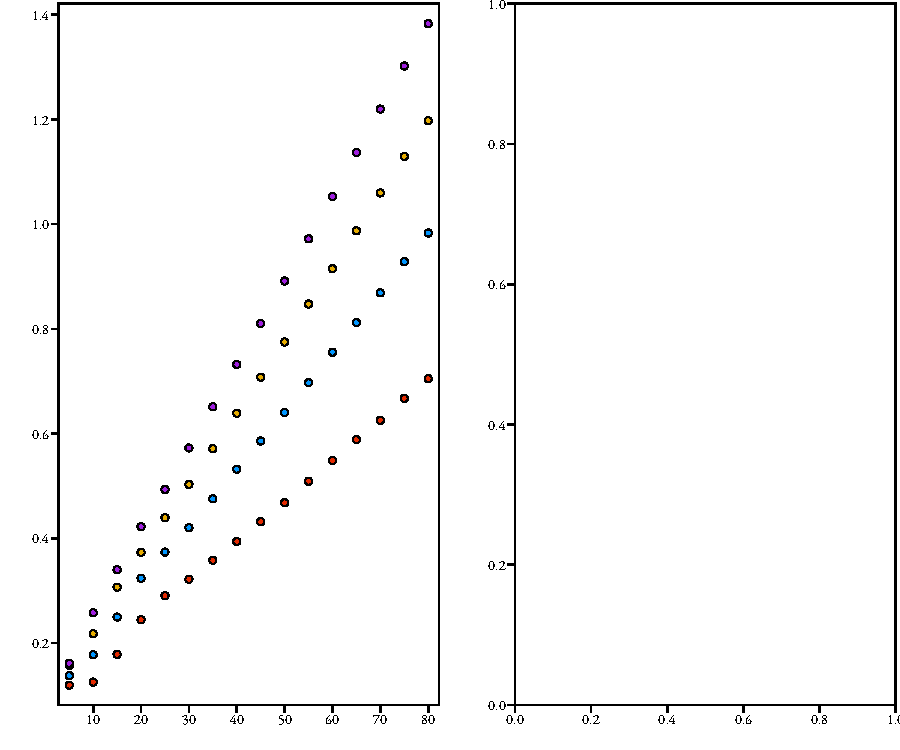
\includegraphics{nlp_profiling/nlp_profiling.pdf}
    \caption[
        The run time and peak memory consumption in computing the Hessian
        matrix for \acsp{FID} with differing numbers of datapoints and signals.
    ]
    {
        The run time and peak memory consumption in computing the Hessian
        matrix for \acsp{FID} with differing numbers of datapoints and signals.
        The \acp{FID} that were used to acquire these results are described in
        the main text.
        \textbf{a1.} and \textbf{b1.} The amount of time required to compute the
        Hessian for \ac{1D} and \ac{2D} \acp{FID}, respectively.
        \textbf{a2.} and \textbf{b2.} Equivalent plots showing the peak memory
        consumption in computing the Hessian.
    }
    \label{fig:nlp-profiling}
\end{figure}
A consideration of the burden on the \ac{CPU} and \ac{RAM} in computing the
Hessian matrix for \ac{1D} and \ac{2D} \acp{FID} (\cref{eq:hess}) is presented in
\cref{fig:nlp-profiling}.
It should be noted that for a typical \ac{NLP} routine, the Hessian will need
to be computed many times (on the order of magnitude of $10^2$ is common) so
while the times presented in the figure may seem small, a rather long total
time is possible for the \ac{NLP} routine if it takes seconds to compute the
Hessian once.
For the \ac{1D} case, simulated \acp{FID} were generated
with both a variable number of contributing signals: $M \in \lbrace 5k : k \in
\lbrace 1, 2, \cdots, 16 \rbrace \rbrace$ and datapoints: $N \in \lbrace 1024k
: k \in \lbrace 1, 2, \cdots, 8 \rbrace \rbrace$. For each \ac{FID}, the Hessian
was computed using a slight variant of the \texttt{obj\_grad\_hess\_1d}
function, given by Lines \ref{ln:objgradhessstart} to
\ref{ln:objgradhessend} in \cref{lst:obj-grad-hess}\footnote{
    The variant of this function neglected the computation of the objective and
    gradient, and returned only the Hessian.
}. There are 4 main steps in computing the Hessian matrix:
\begin{enumerate}
    \item Generation of all the first partial derivatives
        (\cref{eq:first-derivs}), which are stored in a $4M \times N$ array.
    \item Generation of all the non-trivially zero second partial
        derivatives (\cref{eq:second-derivs}), which are stored in a $10M
        \times N$ array.
    \item Computation of the non-zero elements of term \circled{2} in
        \cref{eq:hess}.
    \item Computation term \circled{1} in \cref{eq:hess}.
\end{enumerate}
These steps produce an exact Hessian. Neglecting steps 2 and 3 leads to the
formation of the approximated Hessian as described in
\cref{subsec:hess-approx}. \Cref{fig:nlp-profiling}.a1 shows that the
time to compute the Hessian matrix scales quadratically with $M$, and
linearly with $N$. The cause of this is the fact that the most time-consuming
aspect of the routine is step 4, which involves multiplying the $4M \times N$
matrix of first derivatives with its  $N \times 4M$ conjugate transpose, with a
complexity $\mathcal{O}(M^2N)$. The relative amount of the total run time which
is spent performing step 4 increases steadily as the model order increase, as
seen in \cref{tab:hess-steps}.
As such, for \ac{1D} \acp{FID}, it is
common, especially when the data comprises a large number of
signals, for the discrepancy in the amount of time to compute the true
Hessian relative to its approximation to be small. In these cases, it may be
valuable to compute the exact Hessian if it leads to a reduced number of
required iterations for convergence.
\begin{table}
    \begin{center}
        \begin{tabular}{ c c c c c c }
            \toprule
            $N$/$\Ntwo$ &
            $M$ &
            Step 1 &
            Step 2 &
            Step 3 &
            Step 4 \\
            \midrule
            \multicolumn{6}{c}{\textbf{1D Hessian}}\\
            \midrule
            2048 & 20 & 3.7\% & 9.6\% & 6\% & 76.4\% \\
            8192 & 20 & 3.5\% & 10.7\% & 6.3\% & 75\% \\
            2048 & 80 & 1\% & 3\% & 2\% & 92.6\% \\
            8192 & 80 & 1.2\% & 3.3\% & 1.9\% & 92.4\% \\
            \midrule
            \multicolumn{6}{c}{\textbf{2D Hessian}}\\
            \midrule
            64 & 20 & 8.2\% & 32.5\% & 18.5\% & 38.5\% \\
            256 & 20 & 12.3\% & 50.2\% & 21.3\% & 14.3\% \\
            64 & 80 & 10.8\% & 41\% & 24.3\% & 21.5\% \\
            256 & 80 & 14.9\% & 45.4\% & 24.1\% & 13.8\% \\
            \bottomrule
        \end{tabular}
    \end{center}
    \caption[
        A comparison of the relative times to perform the steps for
        computing the Hessian matrix for \acs{NLP}.
    ]{
        A comparison of the relative times to perform the steps for
        computing the Hessian matrix for \acs{NLP}, for selected pairings of
        $M$ and $N$ (\ac{1D})/$\Ntwo$ (\ac{2D}).
    }
    \label{tab:hess-steps}
\end{table}

To assess the effect of the number of signals and datapoints on Hessian
computation for \ac{2D} \acp{FID}, a series of signals were generated with a
fixed number of datapoints in the first dimension: $\None = 64$. \acp{FID} were
then constructed with the same values of $M$ as the \ac{1D} case, and $\Ntwo
\in \lbrace 64k : k \in \lbrace 1, 2, \cdots, 8 \rbrace \rbrace$. In contrast to
the \ac{1D} case, it is seen that the run time in computing the Hessian now
scales approximately linearly, rather than quadratically. Much more of the run
time is taken up by the first three steps in comparison; computing the
$6M\None\Ntwo$ first derivatives, $21M\None\Ntwo$ second derivatives, and
forming term \circled{2} all scale linearly with $M$, $\None$, and $\Ntwo$. The
relative times spent performing steps 2 and 3 compared with 1 and 4 imply that for
the \ac{2D} case (and for signals more more than 2 dimensions), a large saving
in computational time is typically achieved when the Hessian approximation
is utilised over the exact form.

Both the time- and space-complexity of computing the Hessian is found to be
roughly linear with both $M$ and the number of datapoints in each dimension
for \ac{1D} and \ac{2D} \acp{FID} (see Figures \ref{fig:nlp-profiling}.a2 and
\ref{fig:nlp-profiling}.b2). Most of the \ac{RAM} usage comes from storing
arrays of the first and second partial derivatives. In general, the typical
space requirements for both \ac{1D} and \ac{2D} \acp{FID} should be tolerable
on modern computers, which tend to possess at least \qty{8}{\gibi\byte} of
\ac{RAM}.
